\documentclass[runningheads]{llncs}

\usepackage[T1]{fontenc}
\usepackage[utf8]{inputenc}
\usepackage[brazilian]{babel}
\usepackage{graphicx}
\usepackage{amsmath, amssymb}
\usepackage{booktabs}
\usepackage{subcaption}

\begin{document}

\title{Data Drift em um Modelo Seq2Seq para Predi\c{c}\~ao de Trajet\'orias}

\author{Ivan Yamasaki\inst{1}\orcidID{} \and
Marcos M\'aximo\inst{2}\orcidID{} \and
Paulo Tasinaffo\inst{3}\orcidID{}}
%
\authorrunning{Ivan Yamasaki}
%
\institute{Instituto Tecnol\'ogico de Aeron\'autica, SP, Brasil}
%
\maketitle

\begin{abstract}
Este artigo analisa \textit{data drift} em um modelo \textit{sequence-to-sequence} (seq2seq) para predi\c{c}\~ao de trajet\'orias de rob\^os na RoboCup Small Size League (SSL). O modelo foi treinado com dados de 2019 e avaliado em temporadas posteriores, com foco em dois horizontes de predi\c{c}\~ao. O objetivo \'e medir como o erro, resumido principalmente pelo \textit{Average Displacement Error} (ADE), evolui ao longo do tempo, como essa evolu\c{c}\~ao se compara a um benchmark baseado em filtro de Kalman e em que medida mudan\c{c}as observ\'aveis na din\^amica do jogo acompanham essa degrada\c{c}\~ao.

Os resultados mostram aumento do erro absoluto do seq2seq nos anos posteriores ao treinamento, caracterizando perda de desempenho fora da distribui\c{c}\~ao original. Ao mesmo tempo, a vantagem relativa do seq2seq sobre o Kalman aumenta, sugerindo que ambos sofrem com a mudan\c{c}a temporal dos dados, mas o Kalman degrada mais rapidamente. Como an\'alise complementar, o artigo emprega regress\~oes \textit{Ordinary Least Squares} (OLS) relacionando a varia\c{c}\~ao do ADE com m\'etricas de drift baseadas em Kolmogorov--Smirnov e Wasserstein, controlando efeitos fixos de ano.

Para quantificar a \emph{origem} do drift, o artigo aplica \textit{importance weighting} via LSIF~\cite{kliep}: entre 59\,\% e 72\,\% do excesso de ADE \'e explic\'avel por \emph{covariate shift} nas features cinem\'aticas de entrada, com acelera\c{c}\~ao de cauda (\texttt{accel\_p99}) como dimens\~ao dominante. Uma tentativa de adapta\c{c}\~ao por fine-tuning seletivo \'e avaliada; os resultados indicam que a recupera\c{c}\~ao m\'edia \'e modesta e acompanhada de \emph{catastrophic interference} severo nas trajet\'orias individuais.
\keywords{predi\c{c}\~ao de trajet\'orias \and seq2seq \and data drift \and RoboCup SSL \and Kalman}
\end{abstract}

\section{Introdu\c{c}\~ao}

Predi\c{c}\~ao de trajet\'orias \'e uma tarefa central em sistemas aut\^onomos sujeitos a din\^amica r\'apida. Na RoboCup SSL, prever a movimenta\c{c}\~ao futura dos rob\^os auxilia planejamento, posicionamento e tomada de decis\~ao em tempo real.

O filtro proposto por Kalman~\cite{kalman} \'e tradicional nesse problema por ser simples e barato computacionalmente. No entanto, dependem de hip\'oteses cinem\'aticas restritivas, como din\^amica relativamente suave e bem descrita por modelos lineares locais. Em cen\'arios com acelera\c{c}\~oes bruscas, mudan\c{c}as r\'apidas de dire\c{c}\~ao e estrat\'egias cada vez mais complexas, essa modelagem tende a perder precis\~ao. Al\'em disso, esse tipo de benchmark cinem\'atico n\~ao representa explicitamente inten\c{c}\~oes futuras, intera\c{c}\~oes entre agentes ou ajustes t\'aticos do jogo.

Modelos seq2seq oferecem maior flexibilidade para capturar depend\^encias temporais mais ricas. Eles tamb\'em podem aprender, de forma impl\'icita, padr\~oes recorrentes de a\c{c}\~ao futura a partir dos dados observados, sem precisar explicitar manualmente todas as regras de intera\c{c}\~ao. Por\'em, melhor desempenho em um per\'iodo espec\'ifico n\~ao garante robustez temporal. Se a din\^amica do jogo muda ao longo das temporadas, um modelo treinado em dados antigos pode sofrer degrada\c{c}\~ao ao ser aplicado em anos posteriores. Esse \'e precisamente o problema de \textit{data drift} analisado neste trabalho.

O ponto de partida desta an\'alise \'e o modelo seq2seq originalmente proposto por Lucas Steuernagel e Marcos Ricardo Omena de Albuquerque M\'aximo~\cite{seq2seq} para predi\c{c}\~ao de trajet\'orias na SSL. Assim, a contribui\c{c}\~ao do presente artigo n\~ao est\'a em introduzir uma nova arquitetura, mas em reavaliar temporalmente esse modelo de refer\^encia e investigar sua robustez fora do per\'iodo de treino.

\section{Objetivo}

O objetivo do artigo \'e analisar a robustez temporal de um modelo seq2seq treinado com dados de 2019, considerando dois horizontes de predi\c{c}\~ao, por meio de tr\^es perguntas principais:

\begin{itemize}
    \item como o erro absoluto evolui ao longo do tempo em cada horizonte;
    \item como a diferen\c{c}a de desempenho entre seq2seq e Kalman evolui ao longo dos anos;
    \item se o aumento do erro acompanha m\'etricas observ\'aveis de drift nas vari\'aveis cinem\'aticas.
\end{itemize}

\section{Metodologia}

A an\'alise foi organizada em quatro etapas:

\begin{enumerate}
    \item replica\c{c}\~ao do modelo seq2seq de refer\^encia;
    \item avalia\c{c}\~ao anual do desempenho em temporadas posteriores;
    \item compara\c{c}\~ao com o benchmark de Kalman;
    \item an\'alise estat\'istica complementar da rela\c{c}\~ao entre drift e aumento de erro.
\end{enumerate}

A primeira etapa reproduz o modelo de refer\^encia de Steuernagel e M\'aximo~\cite{seq2seq} com a implementa\c{c}\~ao utilizada neste projeto. Em particular, a entrada de cada passo temporal \'e composta por seis vari\'aveis normalizadas: posi\c{c}\~ao \(x,y\), velocidade \(v_x,v_y\) e orienta\c{c}\~ao codificada por \(\sin(\psi)\) e \(\cos(\psi)\). O treinamento usa uma separa\c{c}\~ao fixa de valida\c{c}\~ao de 10\% dentro do conjunto de treino, \textit{batch size} de 1024, otimizador Adam~\cite{adam}, \textit{early stopping} e redu\c{c}\~ao adaptativa da taxa de aprendizado. Esses detalhes s\~ao mantidos fixos para que a compara\c{c}\~ao temporal reflita mudan\c{c}as na distribui\c{c}\~ao dos dados, e n\~ao mudan\c{c}as no procedimento de ajuste.

A m\'etrica principal \'e o \textit{Average Displacement Error} (ADE), por resumir o desvio m\'edio entre trajet\'oria prevista e trajet\'oria real ao longo do horizonte de predi\c{c}\~ao. Formalmente, para \(N\) trajet\'orias e horizonte \(H\), define-se
\begin{equation}\label{eq:ade}
\mathrm{ADE} = \frac{1}{NH} \sum_{i=1}^{N}\sum_{t=1}^{H} \left\lVert \hat{p}_{i,t} - p_{i,t} \right\rVert_2,
\end{equation}
em que \(\hat{p}_{i,t}\) denota a posi\c{c}\~ao prevista e \(p_{i,t}\) a posi\c{c}\~ao real no instante \(t\) da trajet\'oria \(i\).

Os anos de 2020 e 2021 foram removidos da an\'alise principal. O motivo \'e que esse per\'iodo inclui uma ruptura estrutural relevante no campeonato, especialmente em 2021, quando houve forte mudan\c{c}a de regime. A exclus\~ao evita misturar drift mais gradual com uma altera\c{c}\~ao ex\'ogena do ambiente competitivo.

Ao longo do artigo, os resultados s\~ao apresentados separadamente para os horizontes \(30 \rightarrow 15\) e \(60 \rightarrow 30\).

\section{Arquitetura do modelo}

O modelo utilizado neste trabalho segue uma arquitetura \textit{sequence-to-sequence} do tipo \textit{encoder-decoder} com mecanismo de aten\c{c}\~ao aditiva, em linha com o trabalho de Steuernagel e M\'aximo~\cite{seq2seq} e com o mecanismo de aten\c{c}\~ao popularizado por Bahdanau, Cho e Bengio~\cite{bahdanau}. Na implementa\c{c}\~ao reproduzida aqui, o encoder \'e uma \textit{Long Short-Term Memory} (LSTM) com 128 unidades e o decoder opera de forma auto-regressiva a partir da \'ultima velocidade observada na janela passada.

Considere uma janela passada de comprimento \(n\) e um horizonte futuro de comprimento \(m\), de modo que a entrada e o alvo do modelo se escrevem como
\begin{equation}\label{eq:xy}
X \in \mathbb{R}^{n \times d_x}, \quad Y \in \mathbb{R}^{m \times d_y},
\end{equation}
em que \(d_x\) e \(d_y\) s\~ao, respectivamente, as dimens\~oes da entrada e do alvo em cada instante.

O encoder LSTM processa \(X\) e produz a sequ\^encia de estados ocultos
\begin{equation}\label{eq:enc}
H = [h_1, h_2, \dots, h_n],
\end{equation}
que ser\~ao consultados pelo mecanismo de aten\c{c}\~ao a cada passo do decoder.

Para cada passo \(j\) do decoder, com estado anterior \(s_{j-1}\), define-se primeiro um escore de compatibilidade com cada \(h_k\),
\begin{equation}\label{eq:attn_score}
e_{j,k} = v^{\top} \tanh(W_1\, s_{j-1} + W_2\, h_k),
\end{equation}
que \'e em seguida normalizado por uma \textit{softmax} sobre a janela passada,
\begin{equation}\label{eq:attn_alpha}
\alpha_{j,k} = \frac{\exp(e_{j,k})}{\sum_{\ell=1}^{n} \exp(e_{j,\ell})},
\end{equation}
fornecendo os pesos com que se constr\'oi o vetor de contexto
\begin{equation}\label{eq:attn_ctx}
z_j = \sum_{k=1}^{n} \alpha_{j,k}\, h_k.
\end{equation}

A partir do estado atualizado \(s_j\), o decoder produz a sa\'ida prevista
\begin{equation}\label{eq:dec_out}
\hat{q}_j = W_o\, s_j + b_o,
\end{equation}
e o treinamento minimiza uma perda combinada de erro quadr\'atico m\'edio (\textit{Mean Squared Error}, MSE) e erro absoluto m\'edio (\textit{Mean Absolute Error}, MAE),
\begin{equation}\label{eq:loss}
\mathcal{L} = 100 \cdot (\mathrm{MSE} + \mathrm{MAE}).
\end{equation}

Na configura\c{c}\~ao usada neste projeto, o decoder opera sem \textit{teacher forcing}: a primeira entrada do decoder \'e a \'ultima velocidade observada, e os passos seguintes reutilizam as sa\'idas previamente previstas. Al\'em disso, o pipeline de treinamento parametriza o alvo no espa\c{c}o de velocidades incrementais normalizadas (\texttt{dv}) e reconstr\'oi a trajet\'oria futura em posi\c{c}\~ao a partir do \'ultimo estado observado. Esse detalhe \'e importante porque deixa claro que o modelo n\~ao prev\^e posi\c{c}\~oes diretamente, mas sim uma din\^amica futura que depois \'e acumulada no espa\c{c}o de estados.

\section{Desempenho do seq2seq ao longo do tempo}

A Figura~\ref{fig:ade_por_ano} apresenta a evolu\c{c}\~ao do ADE do seq2seq ao longo dos anos, separadamente para os dois horizontes analisados. Em ambos os casos, o padr\~ao geral ap\'os 2019 \'e de aumento do erro, ainda que com magnitudes distintas.

\begin{figure}
    \centering
    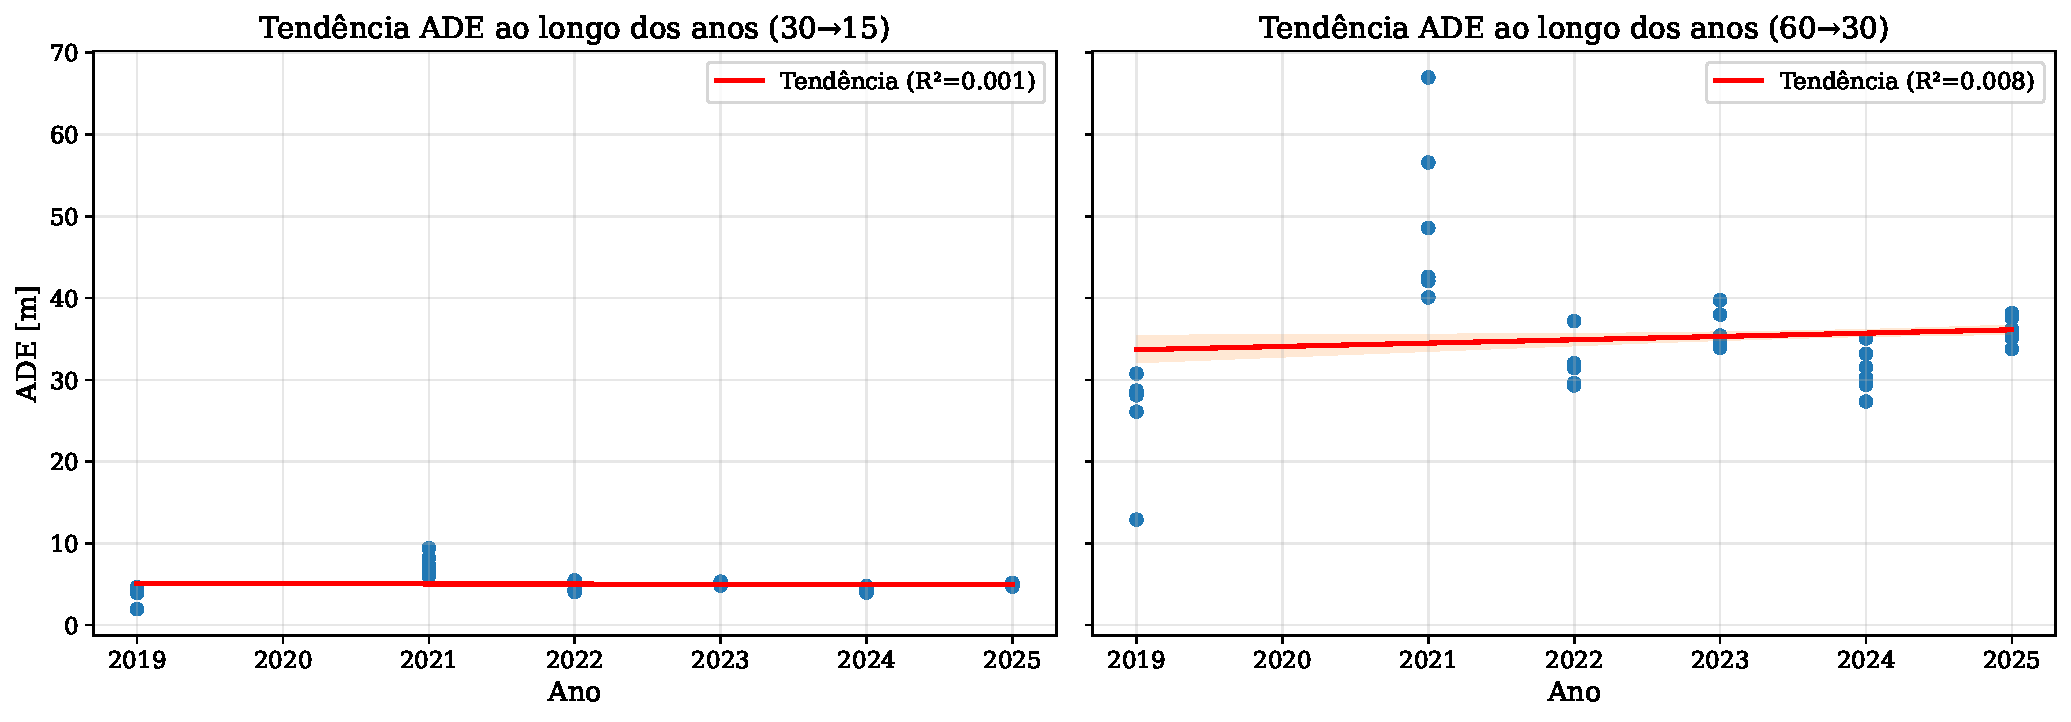
\includegraphics[width=0.95\linewidth]{results/2.ADExYear_pt.pdf}
    \caption{Evolu\c{c}\~ao do ADE do seq2seq ao longo dos anos, separada por horizonte de predi\c{c}\~ao.}
    \label{fig:ade_por_ano}
\end{figure}

Esse resultado \'e consistente com a hip\'otese de \textit{data drift}: o modelo foi treinado em uma distribui\c{c}\~ao associada a 2019 e perde desempenho ao ser aplicado a temporadas posteriores. A separa\c{c}\~ao por horizonte tamb\'em mostra que a deteriora\c{c}\~ao n\~ao \'e necessariamente id\^entica entre tarefas de predi\c{c}\~ao mais curtas e mais longas, o que refor\c{c}a a utilidade de analisar os dois cen\'arios de forma independente.

A leitura desses gr\'aficos deve ser sobretudo descritiva. O objetivo aqui \'e estabelecer o fato b\'asico de que h\'a degrada\c{c}\~ao temporal do erro absoluto do modelo, e n\~ao ainda explicar seu mecanismo.

\section{Compara\c{c}\~ao com o Kalman}

A Figura~\ref{fig:seq_kalman} compara o ADE do seq2seq com o do filtro de Kalman ao longo dos anos, novamente separando os horizontes de predi\c{c}\~ao. O resultado central \'e que o seq2seq permanece melhor do que o Kalman, mas a diferen\c{c}a entre os dois cresce nas temporadas mais recentes.

\begin{figure}
    \centering
    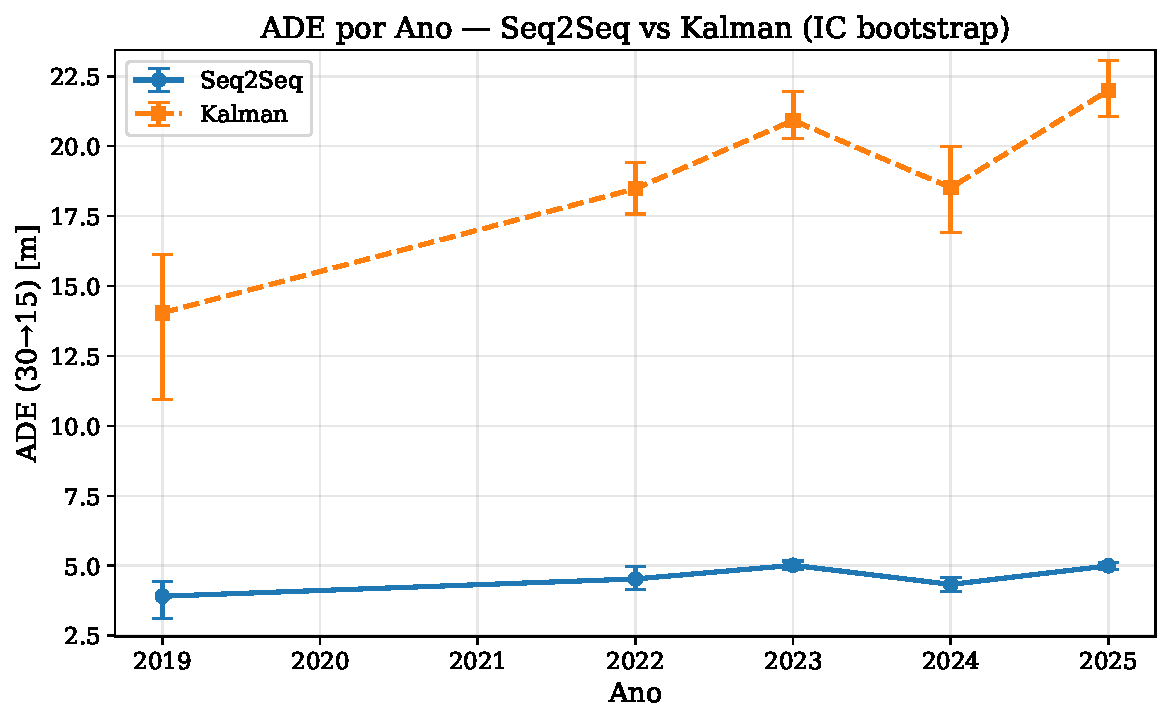
\includegraphics[width=0.95\linewidth]{results/3.Seq2seqVsKalman_pt.pdf}
    \caption{Compara\c{c}\~ao de ADE entre Seq2Seq e Kalman ao longo dos anos, separada por horizonte.}
    \label{fig:seq_kalman}
\end{figure}

Essa evid\^encia precisa ser interpretada com cuidado. O aumento da vantagem relativa do seq2seq n\~ao significa que ele esteja est\'avel. A se\c{c}\~ao anterior j\'a mostrou que o erro absoluto do pr\'oprio seq2seq tamb\'em cresce. A conclus\~ao correta \'e que ambos os m\'etodos sofrem degrada\c{c}\~ao temporal, mas o Kalman parece mais sens\'ivel \`a mudan\c{c}a de distribui\c{c}\~ao.

A Figura~\ref{fig:perc_ade} refor\c{c}a essa interpreta\c{c}\~ao ao mostrar o aumento percentual do ADE de cada m\'etodo em rela\c{c}\~ao a 2019, para cada horizonte. Em praticamente todos os anos analisados, o crescimento percentual do erro do Kalman supera o do seq2seq.

\begin{figure}
    \centering
    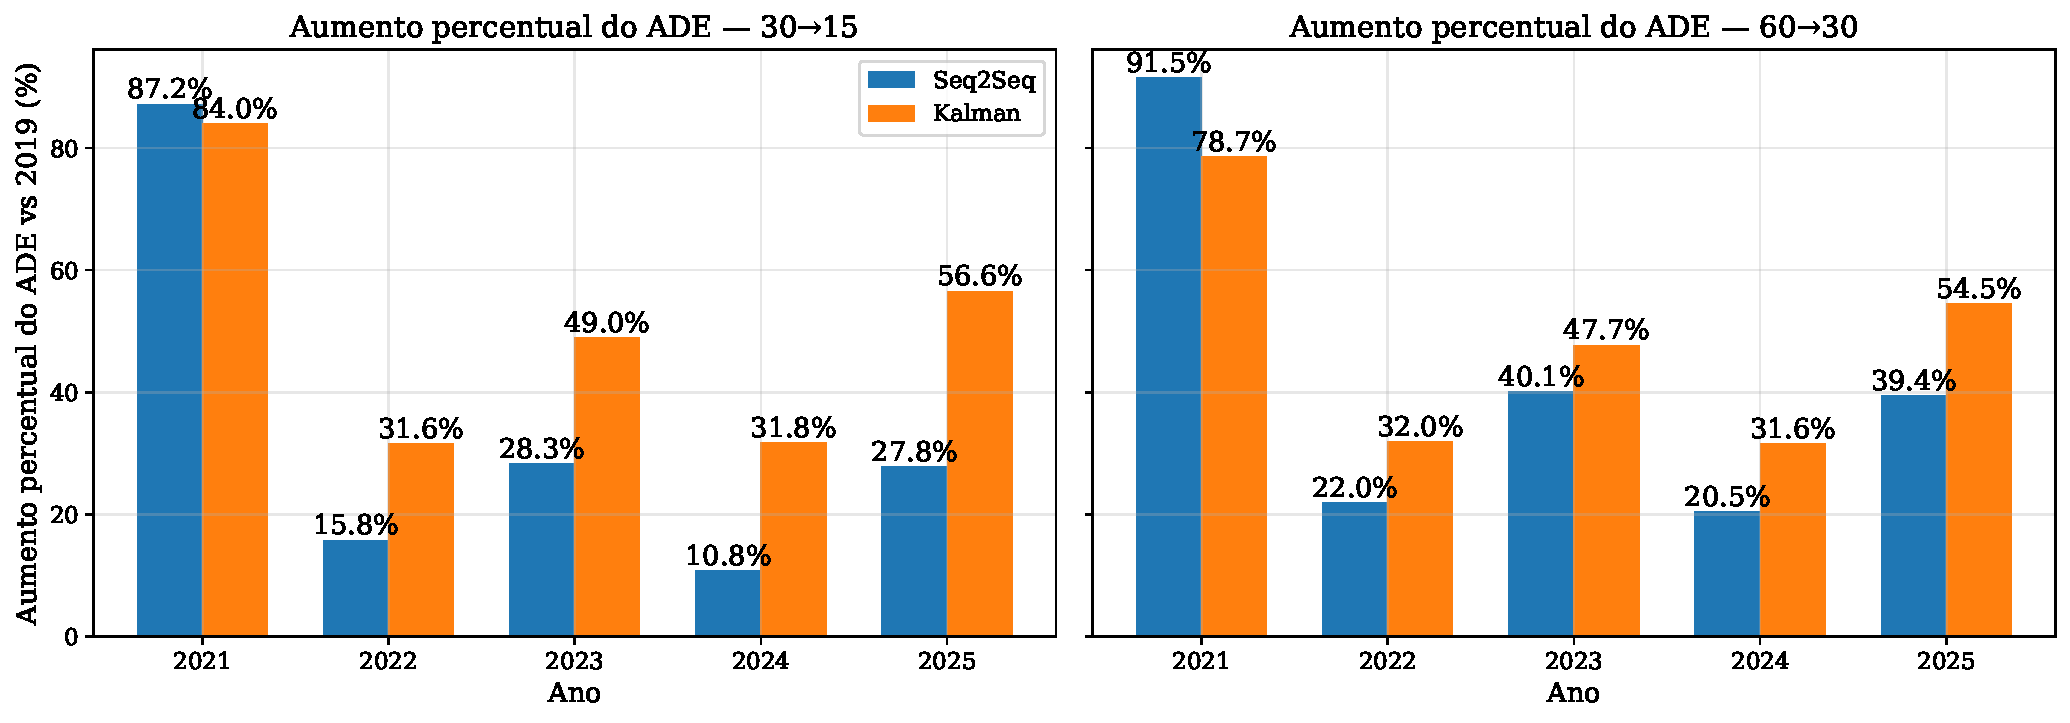
\includegraphics[width=0.95\linewidth]{results/1.PercADE_pt.pdf}
    \caption{Aumento percentual do ADE em rela\c{c}\~ao a 2019 para Seq2Seq e Kalman, separado por horizonte.}
    \label{fig:perc_ade}
\end{figure}

Esse ponto \'e importante porque desloca a leitura do artigo. O resultado principal n\~ao \'e simplesmente que o seq2seq vence o Kalman, mas que ele parece degradar menos quando a din\^amica do jogo se afasta do ambiente de treino. Em termos pr\'aticos, isso sugere maior robustez relativa do modelo neural, ainda que sem eliminar o problema de drift.

\section{Drift nas vari\'aveis cinem\'aticas}

Para investigar poss\'iveis mecanismos por tr\'as da deteriora\c{c}\~ao do desempenho, a Figura~\ref{fig:ks_wd} apresenta a evolu\c{c}\~ao anual de m\'etricas de drift nas vari\'aveis de velocidade, acelera\c{c}\~ao e giro. Foram utilizadas duas fam\'ilias de medidas: estat\'isticas baseadas em Kolmogorov--Smirnov (KS) e dist\^ancias de Wasserstein (WD).

\begin{figure}
    \centering
    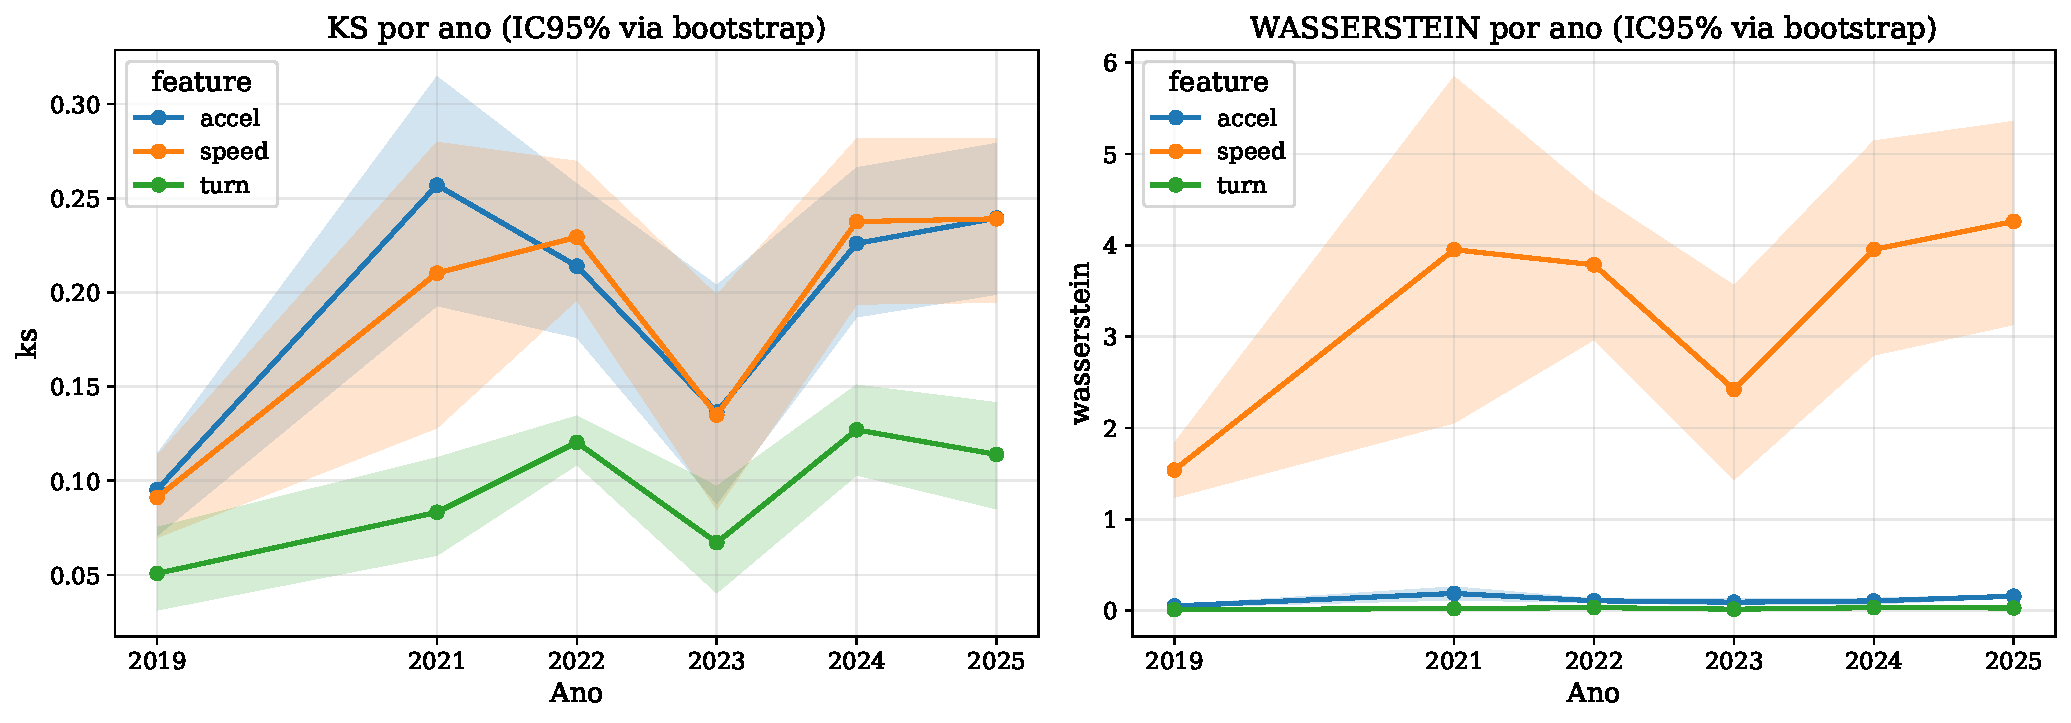
\includegraphics[width=0.95\linewidth]{results/5.KS_WD_xYear_pt.pdf}
    \caption{Evolu\c{c}\~ao anual das m\'etricas KS e WD para vari\'aveis cinem\'aticas.}
    \label{fig:ks_wd}
\end{figure}

Esses gr\'aficos n\~ao provam, por si s\'os, que o drift observado nas vari\'aveis cinem\'aticas cause o aumento do ADE. Ainda assim, eles s\~ao informativos porque mostram que a degrada\c{c}\~ao de desempenho ocorre junto de mudan\c{c}as mensur\'aveis na distribui\c{c}\~ao das vari\'aveis que descrevem a din\^amica do jogo.

Em particular, velocidade e acelera\c{c}\~ao apresentam sinais mais claros de altera\c{c}\~ao nos anos posteriores. Isso \'e compat\'ivel com a hip\'otese de que a SSL passou a exibir partidas mais r\'apidas, com transi\c{c}\~oes mais agressivas e movimentos menos aderentes \`as hip\'oteses simplificadoras do benchmark cl\'assico. A vari\'avel de giro tamb\'em \'e relevante, mas o padr\~ao visual parece menos dominante do que o observado para velocidade e acelera\c{c}\~ao.

\section{An\'alise por regress\~ao OLS}

Como complemento \`a an\'alise descritiva, foram ajustados os seguintes modelos:

\begin{equation}\label{eq:ols_ks}
\Delta ADE \sim ks\_speed + ks\_accel + ks\_turn + C(year),
\end{equation}
\begin{equation}\label{eq:ols_wd}
\Delta ADE \sim wd\_speed + wd\_accel + wd\_turn + C(year).
\end{equation}

Aqui, \(\Delta ADE\) representa a varia\c{c}\~ao do ADE em rela\c{c}\~ao ao ano-base de 2019, enquanto \(C(year)\) introduz efeitos fixos por ano. O papel dessa regress\~ao n\~ao \'e identificar causalidade nem decompor de forma definitiva a origem do erro. A fun\c{c}\~ao da OLS neste artigo \'e mais modesta: verificar se m\'etricas observ\'aveis de drift mant\^em associa\c{c}\~ao com a varia\c{c}\~ao do ADE ap\'os controlar diferen\c{c}as m\'edias entre anos.

A Figura~\ref{fig:ols_ks_wd} apresenta os coeficientes estimados e seus intervalos de confian\c{c}a para cada \textit{feature} de drift, separadamente para os dois horizontes e para as duas fam\'ilias de m\'etricas (KS e WD), permitindo identificar quais vari\'aveis de drift mant\^em associa\c{c}\~ao significativa com \(\Delta ADE\) ap\'os o controle por ano.

\begin{figure}
    \centering
    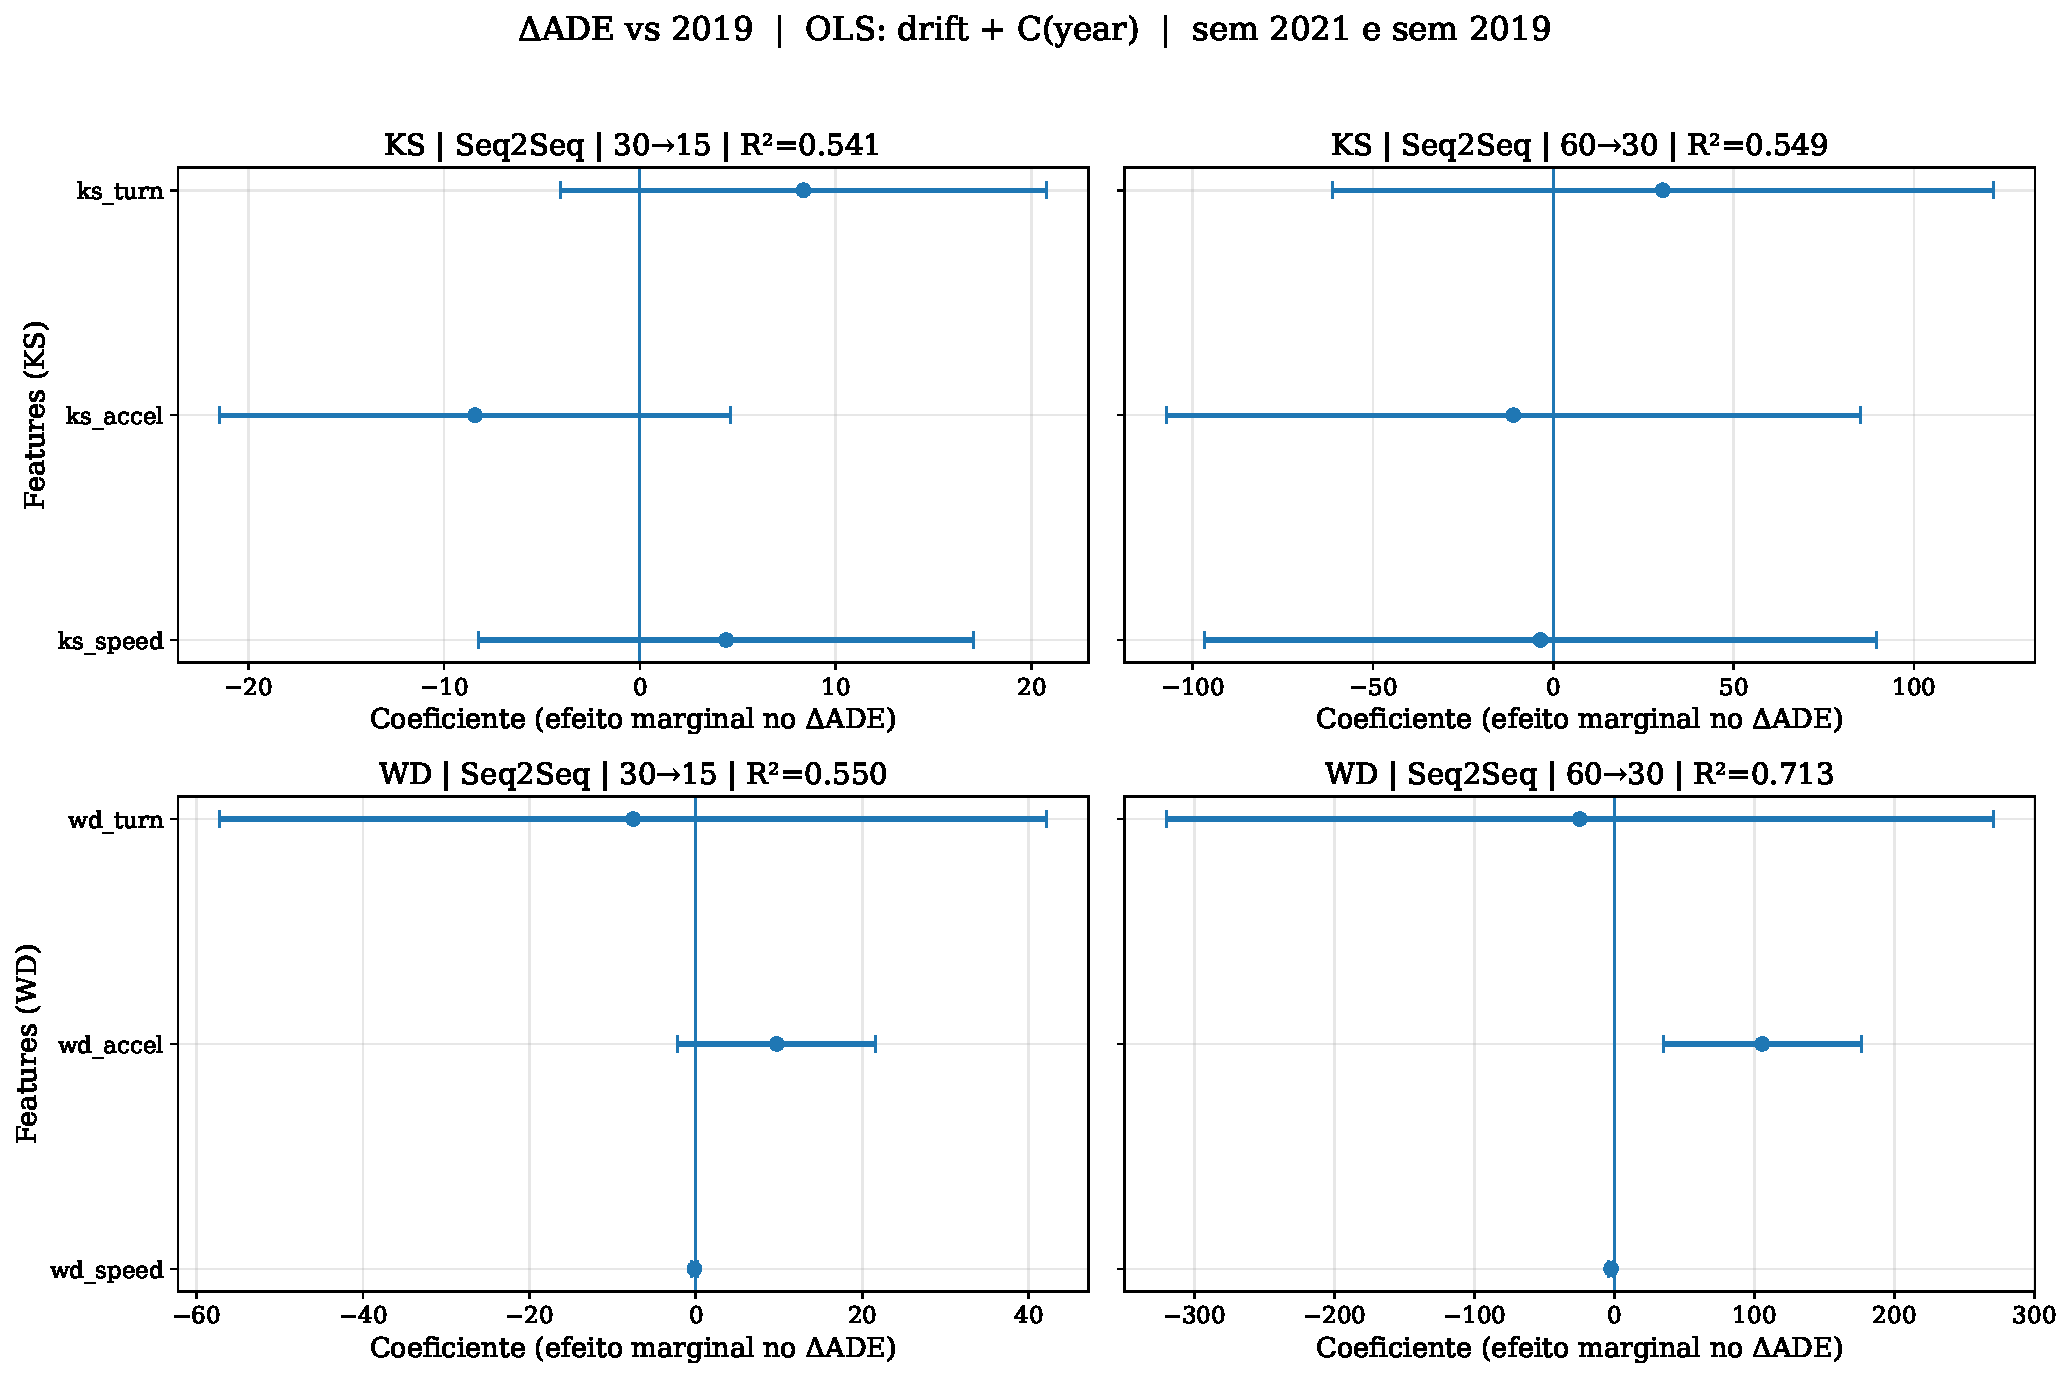
\includegraphics[width=0.9\linewidth]{results/6.OLS_KS_WD_pt.pdf}
    \caption{Resumo visual da an\'alise OLS relacionando \(\Delta ADE\) com m\'etricas de drift.}
    \label{fig:ols_ks_wd}
\end{figure}

A interpreta\c{c}\~ao dessa se\c{c}\~ao exige cautela por pelo menos tr\^es motivos. Primeiro, a an\'alise trabalha com baixa granularidade temporal, o que limita o poder inferencial. Segundo, drift e ano compartilham forte estrutura temporal, de modo que parte da varia\c{c}\~ao carregada pelas m\'etricas KS e WD tamb\'em \'e capturada pelos efeitos fixos anuais. Terceiro, as pr\'oprias m\'etricas de drift podem apresentar correla\c{c}\~ao entre si, especialmente quando descrevem mudan\c{c}as semelhantes nas distribui\c{c}\~oes cinem\'aticas.

Apesar dessas limita\c{c}\~oes, a OLS ainda \'e \'util como exerc\'icio explorat\'orio. Coeficientes positivos para \(ks\_speed\), \(ks\_accel\), \(ks\_turn\) ou seus equivalentes em WD indicam que maior drift nessas vari\'aveis tende a vir acompanhado de maior aumento de erro. Assim, a regress\~ao n\~ao fecha a quest\~ao, mas refor\c{c}a a leitura qualitativa dos gr\'aficos anteriores: a deteriora\c{c}\~ao do ADE n\~ao parece puramente aleat\'oria, e sim associada a mudan\c{c}as observ\'aveis na din\^amica do jogo.

Em outras palavras, esta se\c{c}\~ao deve ser lida como um ponto de partida para uma agenda de infer\^encia mais forte, e n\~ao como sua etapa final. Um pr\'oximo passo natural \'e migrar da an\'alise anual agregada para uma base mais granular, por partida, janela temporal ou bloco de jogadas, permitindo observar varia\c{c}\~ao intra-ano e distinguir melhor o efeito de tempo do efeito do drift mensurado. Com essa granularidade maior, uma estrat\'egia promissora seria modelar explicitamente a exposi\c{c}\~ao ao drift como ``tratamento'' cont\'inuo e estudar sua associa\c{c}\~ao com o erro por meio de um desenho causal mais estruturado, com efeitos fixos e testes de robustez temporal.

\section{Detec\c{c}\~ao formal de drift}

Para complementar a an\'alise descritiva, foram aplicados detectores
formais sobre os streams temporais de ADE e de features cinem\'aticas.
Quatro detectores foram calibrados para o dom\'inio SSL: ADWIN
($\delta=0{,}002$), Page-Hinkley (threshold\,=\,5\,mm), KSWIN
(window\,=\,30, $\alpha=0{,}005$) e Pelt~RBF. Um \emph{null detector}
por permuta\c{c}\~ao ($n=50$) confirmou que os alarmes t\^em $p$-valor
emp\'irico $< 0{,}05$, afastando a hip\'otese de ru\'ido temporal.
O Pelt identificou um \'unico breakpoint inter-ano robusto: transi\c{c}\~ao
2019+2021\,$\to$\,2022, demarcando o ponto a partir do qual o modelo
come\c{c}a a ser avaliado fora de sua distribui\c{c}\~ao efetiva de treino.

\section{Adapta\c{c}\~ao ao drift}

A origem do excesso de ADE foi decomposta via LSIF (\emph{Least-Squares
Importance Fitting})~\cite{kliep}, que estima a raz\~ao de densidades
$\hat{w}(x) = p_{\text{alvo}}(x)/p_{2019}(x)$ sobre as oito features
cinem\'aticas por jogo sem estimar as densidades individualmente.
A \emph{recovery} mede a fra\c{c}\~ao do excesso total atribu\'ida a
\emph{covariate shift}:
\begin{equation}\label{eq:recovery}
\mathrm{recovery}(y) =
    \frac{\mathrm{ADE}_y - \mathrm{ADE}_{\mathrm{IW}}(y)}
         {\mathrm{ADE}_y - \mathrm{ADE}_{2019}} \times 100\,\%.
\end{equation}

Para os anos com excesso positivo (2021, 2022, 2023, 2025), a recovery
ficou entre 59\,\% e 72\,\% (IC\,95\,\% via bootstrap; $n=48\,000$
trajet\'orias por ano), com mediana $\approx 63\,\%$. O ESS ratio acima de
0{,}57 em todos os casos confirma a estabilidade do estimador. A feature
dominante \'e \texttt{accel\_p99}: usada isoladamente, explica mais de
50\,\% do excesso em todos os anos analisados e seu ranking estabiliza
entre temporadas.

Uma tentativa de adapta\c{c}\~ao por fine-tuning seletivo (encoder
congelado, 2 camadas do decoder descongeladas, lr\,=\,$10^{-5}$, early-stop
por \texttt{cat\_ratio}) reduziu o ADE m\'edio em apenas $0{,}13$\,mm
($-2{,}7\,\%$), com recovery\,=\,32{,}7\,\%. O \texttt{cat\_ratio}\,=\,0{,}82
j\'a na 1\textordfeminine{} \'epoca indica que a melhora na m\'edia vem \`a custa
de degrada\c{c}\~ao severa em trajet\'orias individuais: para cada trajet\'oria
melhorada, 0{,}82 foram pioradas. A valida\c{c}\~ao por divis\~ao confirmou
que o drift \'e real e intra-divis\~ao (todos os dados p\'os-2021 pertencem
\`a Divis\~ao\,A; Divis\~ao\,B ausente no conjunto de dados).

\section{Discuss\~ao}
Os resultados do artigo apontam para tr\^es mensagens principais.

A primeira \'e a mais s\'olida: o seq2seq sofre degrada\c{c}\~ao temporal de desempenho. O aumento do ADE em anos posteriores ao treinamento \'e consistente com presen\c{c}a de \textit{data drift}.

A segunda tamb\'em \'e robusta: a vantagem relativa do seq2seq sobre o Kalman cresce ao longo do tempo. Isso sugere que o benchmark cl\'assico \'e ainda mais sens\'ivel \`as mudan\c{c}as de regime da SSL. Logo, robustez relativa maior n\~ao implica aus\^encia de drift; implica apenas deteriora\c{c}\~ao menos acentuada.

A terceira mensagem \'e mais moderada: parte dessa varia\c{c}\~ao do erro parece acompanhar medidas observ\'aveis de drift nas vari\'aveis cinem\'aticas. Essa conclus\~ao \'e sustentada pela combina\c{c}\~ao entre leitura visual das s\'eries de KS e WD e pela an\'alise OLS, mas ainda deve ser entendida como evid\^encia sugestiva, n\~ao conclusiva.

Essa distin\c{c}\~ao \'e importante para a interpreta\c{c}\~ao do artigo. A contribui\c{c}\~ao principal do trabalho \'e emp\'irica e diagn\'ostica: mostrar que o desempenho fora do per\'iodo de treino se deteriora e que essa deteriora\c{c}\~ao \'e consistente com mudan\c{c}a de distribui\c{c}\~ao. A parte econom\'etrica entra como apoio anal\'itico, ajudando a organizar hip\'oteses sobre o mecanismo do drift, mas sem ainda resolv\^e-las de forma causal.

A an\'alise por importance weighting adiciona uma quarta mensagem: o drift \'e predominantemente covariate. A mediana de recovery $\approx 63\,\%$ indica que corrigir a distribui\c{c}\~ao de entrada pelo LSIF recupera cerca de dois ter\c{c}os do excesso de ADE, com \texttt{accel\_p99} como dimens\~ao dominante. O ter\c{c}o restante ($\approx 37\,\%$) n\~ao \'e explicado por covariate shift, sugerindo algum concept drift residual que n\~ao pode ser corrigido por repondera\c{c}\~ao. Do lado da adapta\c{c}\~ao, os experimentos de fine-tuning mostram que a simples atualiza\c{c}\~ao dos pesos do decoder n\~ao resolve o problema: o \emph{catastrophic interference} \'e imediato e severo. Esses resultados combinados configuram o Cen\'ario~3 descritivo: o drift \'e real, detectado formalmente e parcialmente explic\'avel, mas a adapta\c{c}\~ao efetiva requer estrat\'egias mais sofisticadas do que fine-tuning padr\~ao.

Tamb\'em \'e importante delimitar com clareza o escopo da contribui\c{c}\~ao frente ao artigo de Steuernagel e M\'aximo~\cite{seq2seq}. O presente trabalho herda desse artigo o n\'ucleo arquitetural do preditor neural e o benchmark comparativo com Kalman. O avan\c{c}o aqui est\'a em deslocar a pergunta de pesquisa: em vez de perguntar apenas se o seq2seq supera o benchmark em um recorte fixo, pergunta-se como esse ganho evolui quando a distribui\c{c}\~ao temporal dos dados se afasta do ambiente de treino.

Nesse sentido, uma agenda natural de continuidade seria investigar diretamente se o drift afeta mais o seq2seq ou o Kalman em magnitude marginal. Em vez de modelar apenas o erro absoluto, uma extens\~ao interessante \'e usar como vari\'avel dependente a diferen\c{c}a \(ADE^{Kalman} - ADE^{Seq2Seq}\) ou sua raz\~ao relativa. Isso permitiria estudar n\~ao apenas se h\'a drift, mas em que contextos ele amplia mais a vantagem comparativa do modelo neural sobre o benchmark cl\'assico.

\section{Conclus\~ao}

Este artigo analisou a estabilidade temporal de um modelo seq2seq para predi\c{c}\~ao de trajet\'orias na RoboCup SSL. Os resultados mostram que o modelo perde desempenho em anos posteriores ao treinamento, caracterizando drift. Tamb\'em mostram que o aumento relativo do erro do Kalman \'e maior, o que amplia a vantagem comparativa do seq2seq em temporadas mais recentes.

Portanto, a conclus\~ao principal \'e dupla. Primeiro, h\'a evid\^encia clara de degrada\c{c}\~ao temporal no seq2seq. Segundo, o Kalman parece sofrer ainda mais com a mudan\c{c}a temporal da distribui\c{c}\~ao dos dados. As m\'etricas KS e WD, juntamente com a an\'alise OLS, refor\c{c}am a interpreta\c{c}\~ao de que o aumento do erro acompanha mudan\c{c}as mensur\'aveis na din\^amica observada das partidas.

Ao mesmo tempo, o artigo delimita o alcance dessa infer\^encia. A regress\~ao OLS deve ser lida como an\'alise explorat\'oria complementar, \'util para orientar hip\'oteses e pr\'oximos testes, mas insuficiente para sustentar causalidade.

A quantifica\c{c}\~ao via LSIF revelou que \texttt{accel\_p99} \'e a feature de covariate shift dominante, com ranking est\'avel entre temporadas. Isso sugere que a SSL passou a exibir partidas com din\^amica de acelera\c{c}\~ao mais agressiva ao longo dos anos, e que esse \'e o principal vetor de degrada\c{c}\~ao do modelo. Uma agenda natural de continuidade seria, portanto, incorporar essa dimens\~ao diretamente no modelo, seja como feature de condi\c{c}\~ao do encoder, seja via retrining incremental com estrat\'egias que mitiguem \emph{catastrophic interference} (e.g., EWC, replay de trajet\'orias de treino, ou adapta\c{c}\~ao do encoder em vez de apenas do decoder). Em termos de cr\'edito cient\'ifico, o presente estudo se apoia diretamente na linha inaugurada por Steuernagel e M\'aximo~\cite{seq2seq}, estendendo-a do problema de desempenho pontual para o problema de estabilidade temporal e adapta\c{c}\~ao ao drift.

\begin{thebibliography}{9}

\bibitem{seq2seq}
Steuernagel, L., M\'aximo, M. R. O. A.: Trajectory Prediction for SSL Robots Using Seq2seq Neural Networks. In: Eguchi, A., Lau, N., Paetzel-Pr\"usmann, M., Wanichanon, T. (eds.) RoboCup 2022: Robot World Cup XXV. LNCS, vol. 13561, pp. 27--38. Springer, Cham (2023). doi:10.1007/978-3-031-28469-4\_4

\bibitem{bahdanau}
Bahdanau, D., Cho, K., Bengio, Y.: Neural Machine Translation by Jointly Learning to Align and Translate. In: 3rd International Conference on Learning Representations (ICLR) (2015)

\bibitem{kalman}
Kalman, R. E.: A New Approach to Linear Filtering and Prediction Problems. Journal of Basic Engineering \textbf{82}(1), 35--45 (1960)

\bibitem{adam}
Kingma, D. P., Ba, J.: Adam: A Method for Stochastic Optimization. In: 3rd International Conference on Learning Representations (ICLR) (2015)

\bibitem{kliep}
Sugiyama, M., Nakajima, S., Kashima, H., von B\"unau, P., Kawanabe, M.: Direct importance estimation with model selection and its application to covariate shift adaptation. In: Advances in Neural Information Processing Systems (NIPS) (2008)

\bibitem{sugiyama_book}
Sugiyama, M., Kawanabe, M.: Machine Learning in Non-Stationary Environments: Introduction to Covariate Shift Adaptation. MIT Press (2012)

\end{thebibliography}

\end{document}
